% SPDX-License-Identifier: GPL-3.0-or-later OR CC-BY-SA-4.0
\section{Main Page}\label{sec:main-page} %%##pages_mainpage-section==title>>
%%!!pages_mainpage-section<<
Main page lists all the installed, uninstalled and backed up applications. A single click on any installed app item
opens the respective \hyperref[sec:app-details-page]{App Details page}. For the uninstalled system apps, it displays a
dialog prompt which can be used to reinstall the app. Using the \hyperlink{par:main-page-sort}{sort} option from the
list options, the app items can be sorted in various ways and preserved on exit. It is also possible to filter items
using the \hyperlink{par:main-page-filter}{filter} option in the list options. Filtering is possible also via the search
bar with additional support for the regular expressions.
%%!!>>

\begin{figure}[ht]
    \centering
    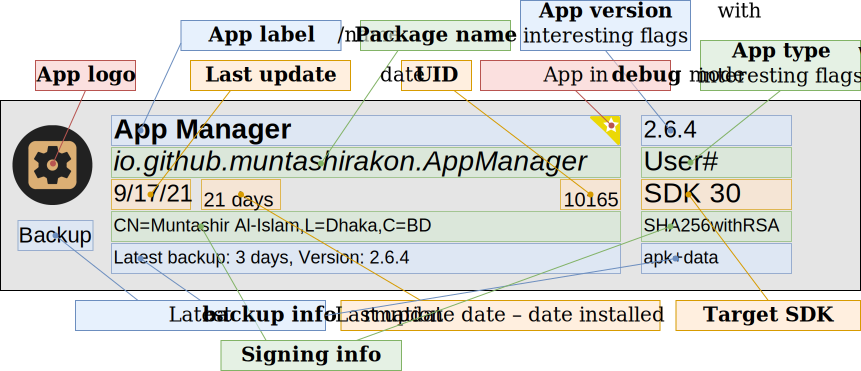
\includegraphics{./images/main_page_entry_info_labeled.svg}
    \caption{An application list item in the main page} %%##pages_mainpage-howappopswork==title>>
    \label{fig:main_page_entry_info_labeled}
\end{figure}

\subsection{Batch Operations}\label{subsec:batch-operations} %%##pages_mainpage-batch-operations==title>>
%%!!pages_mainpage-batch-operations<<
Batch operations or operation on multiple applications are also available within this page. Multiple selection mode can
be activated by clicking on any app icon or by long-clicking on any items in the list. Once activated, a single click on
a list item selects it instead of opening the App Details page. In this mode, the batch operations are located in the
multiple selection menu at the bottom of the page. The operations include:
\begin{itemize}
    \item Adding the selected applications to a \hyperref[sec:profiles-page]{profile}
    \item \hyperref[sec:backup-restore]{Backing up, restoring or deleting} the applications
    \item Blocking the trackers from the applications
    \item Clearing data or cache from the applications
    \item Enabling/disabling/force-stopping/uninstalling the applications
    \item Exporting the blocking rules saved inside App Manager
    \item Preventing the background operations of the applications (Android 7 and onwards)
    \item Saving the APK files to \texttt{AppManager/apks}
    \item Setting \hyperref[sec:net-policy]{net policies}
\end{itemize}

\begin{tip}{Accessibility}
    After the multiple selection mode has been activated, it is possible to navigate in or out of the multiple selection
    menu using the right or left keys of the keyboard or remote.
\end{tip}
%%!!>>

\subsection{Colour Codes}\label{subsec:main-colour-codes} %%##pages_mainpage-colour-codes==title>>
%%!!pages_mainpage-colour-codes<<
\begin{itemize}
    \item \colorbox{AMLightGreyishOrange}{\textcolor{black}{Light greyish orange (day)}} / \colorbox{AMDarkBlue}{
        \textcolor{white}{dark blue (night)}} -- The application is selected for batch operation
    \item \colorbox{AMLightRed}{\textcolor{black}{Light red (day)}} / \colorbox{AMVeryDarkRed}{\textcolor{white}
    {dark red (night)}} -- Disabled app
    \item \colorbox{AMYellow}{\textcolor{black}{Yellow Star}} -- Debuggable application
    \item \textcolor{AMOrange}{Orange \textit{Date}} -- The app has access to the system logs
    \item \textcolor{AMOrange}{Orange \textit{UID}} -- The user ID is being shared among multiple applications
    \item \textcolor{AMOrange}{Orange \textit{SDK}} -- The application possibly uses cleartext (ie. HTTP) traffic
    \item \textcolor{red}{Red \textit{package name}} -- The application does not allow clearing its data
    \item \textcolor{red}{Red \textit{backup}} -- The uninstalled application with one or more backups present in App
    Manager
    \item \textcolor{AMOrange}{Orange \textit{backup}} -- Outdated backup, i.e.\ the base backup contains an older
    version of the installed application
    \item \textcolor{AMDarkCyan}{Dark cyan \textit{backup}} -- Up to date backup, i.e.\ the base backup contains the
    same or higher version of the installed application
    \item \textcolor{AMDarkCyan}{Dark cyan \textit{package name}} -- Force-stopped application
    \item \textcolor{AMDarkCyan}{Dark cyan \textit{version}} -- Inactive application
    \item \textcolor{magenta}{Magenta} -- Persistent application i.e.\ it remains running all the time.
\end{itemize}
%%!!>>

\subsection{Application Types}\label{subsec:main-page-application-types} %%##pages_mainpage-application-types==title>>
%%!!pages_mainpage-application-types<<
An application can be either a \textbf{User} or a \textbf{System} application along with the following suffixes:
\begin{itemize}
    \item \texttt{X} -- Supports multiple architectures
    \item \texttt{0} -- No dex files present in the application
    \item \texttt{\textdegree°} -- Suspended application
    \item \texttt{\#} -- The application requested the system to allocate a large heap i.e. large runtime memory
    \item \texttt{?} -- The application requested the virtual machine to be in the safe mode.
\end{itemize}
%%!!>>

\subsection{Version Info}\label{subsec:main-page-version-info} %%##pages_mainpage-version-info==title>>
%%!!pages_mainpage-version-info<<
Version name is followed by the prefixes below:
\begin{itemize}
    \item \texttt{\_} -- No hardware acceleration (breaking the in-app animations or transparencies)
    \item \texttt{\textasciitilde} -- Test-only application
    \item \texttt{debug} -- Debuggable application
\end{itemize}
%%!!>>

\subsection{Options Menu}\label{subsec:main-page-options-menu} %%##pages_mainpage-options-menu==title>>
%%!!pages_mainpage-options-menu<<
Options menu offers several options that can be used to sort and filter the listed applications as well as to navigate
to different pages within or outside App Manager.
%%!!>>

\subsubsection{Instructions} %%##pages_mainpage-instructions==title>>
%%!!pages_mainpage-instructions<<
Clicking on the \textbf{Instructions} opens the offline version of the App Manager user manual. It may also open the
online version if the corresponding feature split i.e.\ \texttt{feat\_docs} is not installed, or if an WebView is not
present in the system to load the manual.
%%!!>>

\subsubsection{List Options}\label{subsubsec:main-list-options} %%##pages_mainpage-list-options==title>>
%%!!pages_mainpage-list-options<<
\textbf{List options} contain the options to sort and filter the list in the main page.
%%!!>>

\paragraph{Sort}\hypertarget{par:main-page-sort}{} %%##pages_mainpage-sort==title>>
%%!!pages_mainpage-sort<<
The applications listed in the main page can be sorted in the following ways:
\begin{itemize}
    \item \textbf{User apps first.} The user applications are listed on the top
    \item \textbf{App label.} Sort the list in ascending order based on their application labels (also known as
    \textit{application names}). This is the default sorting preference
    \item \textbf{Package name.} Sort the list in ascending order based on their package names
    \item \textbf{Last update.} Sort the list in descending order based on the date they were last updated
    \item \textbf{Shared user ID.} Sort the list in descending order based on their kernel user ID
    \item \textbf{Target SDK.} Sort the list in ascending order based on their target SDK
    \item \textbf{Signature.} Sort the list in ascending order based on their signing information
    \item \textbf{Disabled first.} The disabled applications are listed on the top
    \item \textbf{Blocked first.} Sort the list in descending order based on the number of blocked components each
    application has
    \item \textbf{Backed up first.} Display the applications with backups on the top
    \item \textbf{Trackers.} Sort the list in descending order based on the number of tracker components each
    application has
    \item \textbf{Last actions.} Sort the list in descending order based on the latest time and date of any actions made
    to the applications within App Manager.
\end{itemize}

In addition, there is the \textit{reverse} option that can be used to sort the list in the reverse order. Regardless of
the sorting preferences, the applications are sorted alphabetically at first in order to prevent producing any random
sorting results.
%%!!>>

\paragraph{Filter}\hypertarget{par:main-page-filter}{} %%##pages_mainpage-filter==title>>
%%!!pages_mainpage-filter<<
The applications listed in the main page can be filtered in the following ways:
\begin{itemize}
    \item \textbf{User apps.} List only the user applications
    \item \textbf{System apps.} List only the system applications
    \item \textbf{Disabled apps.} List only the disabled applications
    \item \textbf{Apps with rules.} List the applications with one or more blocking rules
    \item \textbf{Apps with activities.} List the applications with one or more activities
    \item \textbf{Apps with backups.} List the applications with one or more backups
    \item \textbf{Running apps.} List the applications that are currently running
    \item \textbf{Apps with splits.} List the applications with one or more split APK files
    \item \textbf{Installed apps.} List only the installed applications
    \item \textbf{Uninstalled apps.} List only the uninstalled applications
    \item \textbf{Apps without backups.} List the applications with no backups present.
\end{itemize}

Unlike sorting, it is possible to apply more than one filtering options at the same time. For example, the disabled user
applications can be listed by selecting both \textit{User apps} and \textit{Disabled apps}. This can be particularly
useful for \hyperref[subsec:batch-operations]{batch operations} where filtering the user applications may be necessary
to carry out certain operations safely.
%%!!>>

\paragraph{Profile Name}%%##pages_mainpage-profile_name==title>>
%%!!pages_mainpage-profile_name<<
It is also possible to list the applications that are only present in a \hyperref[sec:profiles-page]{profile}. This can
be useful for carrying out certain operations on a profile (e.g., uninstalling all the applications in a profile) that
cannot be done via the \hyperref[sec:profiles-page]{Profiles page}.
%%!!>>

\subsubsection{1-Click Ops}\label{subsubsec:main:1-click-ops} %%##pages_mainpage-1-click-ops==title>>
%%!!pages_mainpage-1-click-ops<<
\textbf{1-Click Ops} stands for the single-click operations. It opens the \hyperref[sec:1-click-ops-page]{corresponding
page} in a new activity.
%%!!>>

\subsubsection{App Usage} %%##pages_mainpage-appusage==title>>
%%!!pages_mainpage-appusage<<
App usage statistics such as \textit{screen time}, \textit{data usage} (both mobile and Wi-Fi), \textit{the number of
times an app was opened} can be accessed by clicking on the \textbf{App Usage} option in the menu. However, it requires
the \textit{Usage Access} permission. This menu item will not be listed if the usage access feature is disabled in
\hyperref[subsec:enable/disable-features]{settings}.
%%!!>>

\subsubsection{System Config} %%##pages_mainpage-systemconfig==title>>
%%!!pages_mainpage-systemconfig<<
This menu item opens a new page where various system configurations, blacklists/whitelists included in Android by the
OEM, the vendor, the AOSP or the Magisk modules are displayed. It requires root. Therefore, this menu item will not be
listed if root permission is unavailable to App Manager.
%%!!>>

\subsubsection{Running Apps}\label{subsubsec:main:running-apps} %%##pages_mainpage-running-apps==title>>
% TODO: Create a new page for the running apps
%%!!pages_mainpage-running-apps<<
This menu item opens a new page where a list of running applications or processes are displayed. It also displays the
current memory and cache (if available) usage. If root or ADB is not available to App Manager, it only displays itself
in the recent versions of Android. The running applications or processes can also be force-stopped or killed within the
resultant page. Logs for each process ID (PID) can also be viewed in the \hyperref[subsubsec:log-viewer]{log viewer}.
In addition, it is also possible to carry out batch operations either by clicking on the icon or by long-clicking on an
item. Normal click on any items opens a dialog where a more detailed information is displayed.
%%!!>>

\subsubsection{Profiles} %%##pages_mainpage-profiles==title>>
%%!!pages_mainpage-profiles<<
This menu item opens the \hyperref[sec:profiles-page]{profiles page}. Profiles are a way to configure regularly used
tasks. They can also be invoked via shortcuts.
%%!!>>

\subsubsection{Log Viewer}\label{subsubsec:log-viewer} %%##pages_mainpage-log-viewer==title>>
% TODO: Create a new page for the log viewer
%%!!pages_mainpage-log-viewer<<
This menu item opens the log viewer page which can display and manage logs using the \texttt{logcat} command. By
default, this page can only display the activities of App Manager. However, it can display logs from all the
processes if \texttt{android.permission.READ\_LOGS} is granted. This permission granted automatically if the current
\hyperref[subsec:mode-of-operation]{mode of operation} is either root or ADB.
%%!!>>

\subsubsection{APK Updater} %%##pages_mainpage-apkupdater==title>>
%%!!pages_mainpage-apkupdater<<
If the app \href{https://github.com/rumboalla/apkupdater}{APK Updater} is installed in the system, it can be opened
directly via this menu item. The option remains hidden if the app is not present in the system.
%%!!>>

\subsubsection{Termux} %%##pages_mainpage-termux==title>>
%%!!pages_mainpage-termux<<
If the app \href{https://github.com/termux/termux-app}{Termux} is installed in the system, the running session (or a
new session) can be opened directly via this menu item. The option remains hidden if the app is not present in the
system.
%%!!>>

\subsubsection{Settings} %%##pages_mainpage-settings==title>>
%%!!pages_mainpage-settings<<
This menu item opens the in-app \hyperref[sec:settings-page]{Settings page}.
%%!!>>
